\documentclass{article}

\usepackage{tikz}
\usetikzlibrary{positioning}

\title{Interaction Diagram - Find Books With Tag}
\author{Nicholas Riesen}

% no page number at bottom
\pagenumbering{gobble}

\begin{document}
\maketitle

\begin{center}
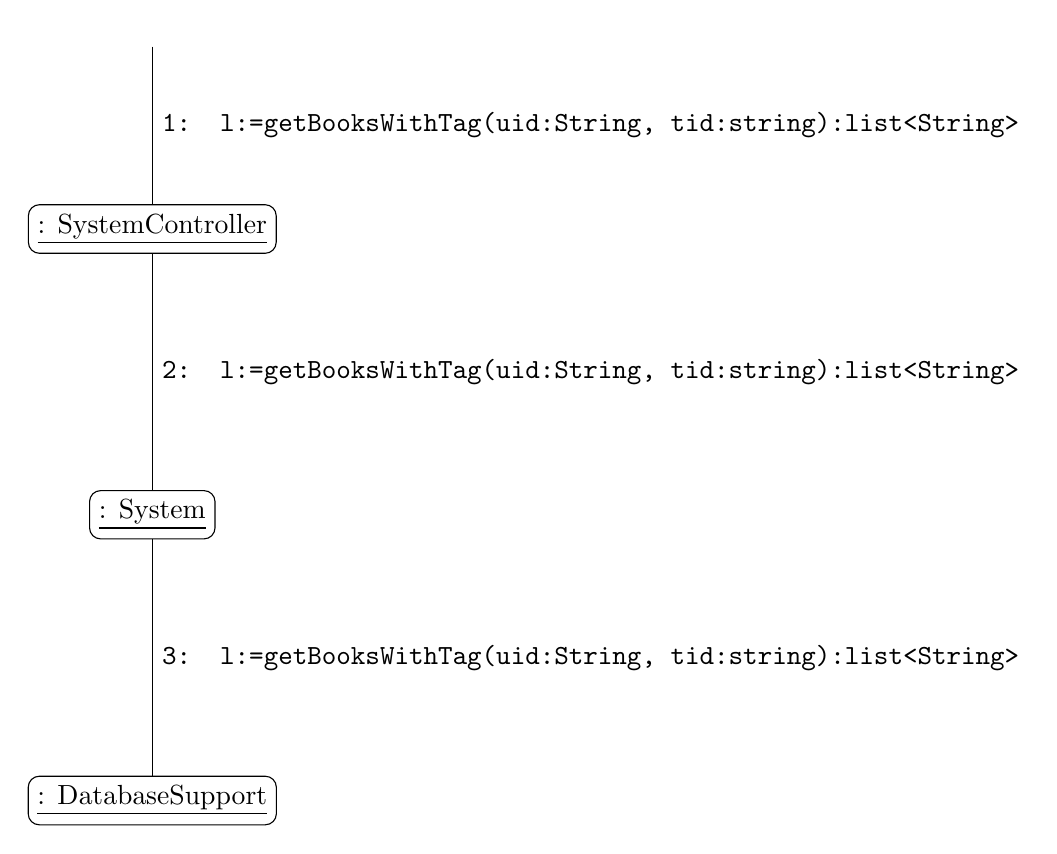
\begin{tikzpicture}[
  auto,
  block/.style = {
    rectangle,
    draw=black,
    align=center,
    rounded corners
  }
]

\node[] (start) {};

\node[block, below = 2cm of start]      (controller) {\underline{: SystemController}};
\node[block, below = 3cm of controller] (system)     {\underline{: System}}; 
\node[block, below = 3cm of system]     (database)   {\underline{: DatabaseSupport}};

\draw (start)      -- (controller) node[midway] {\texttt{1: l:=getBooksWithTag(uid:String, tid:string):list<String>}};
\draw (controller) -- (system)     node[midway] {\texttt{2: l:=getBooksWithTag(uid:String, tid:string):list<String>}};
\draw (system)     -- (database)   node[midway] {\texttt{3: l:=getBooksWithTag(uid:String, tid:string):list<String>}};

\end{tikzpicture}
\end{center}

\end{document}
